\chapter{Limits and Differentiation}

In this chapter, we will continue to develop the theory of complex functions in a way that mirrors your first introduction to calculus. Now that we know what our functions of interest are, let's talk about limits and differentiation.

\section{Limits}

Just like for differentiation over $\R$, our first building block is the limit. There is a complication here though: in $\R$, when we take a limit we're looking at two directions: $\lim_{x\rightarrow c} f(x)$ depends on what $f(x)$ does as $x$ approaches $c$ from the left hand and from the right hand.

In $\C$, we not longer have two directions. We have an infinite number! More than that though, we need to consider not just travelling along straight lines, but rather any curve toward our point.

To capture this, I'll present two definitions. The first is a fairly formal one, and we aren't going to work with it at all. It may appear in some proofs, but that's all. The second is the intuitive way to understand limits.

\begin{defbo}{$\varepsilon$-$\delta$ Definition of a Limit}{limitde}
\index{Limit!formal definition}
Let $U\subset \C$, $z_0 \in \C$, and $f:U\rightarrow \C$. Further, assume there exists some $r > 0$ such that $\{z\in \C| 0 < |z-z_0| < r\} \subset U$. Then $\displaystyle\lim_{z\rightarrow z_0} f(z) = L$ if:
$$\forall \varepsilon > 0, \exists \delta \text{ such that } 0 < |z-z_0| < \delta \implies |f(z) - L| < \varepsilon$$
\end{defbo}

Intuitively, this says that for any $\varepsilon > 0$, we can find a circle around $z_0$ so that if $z$ is inside this circle, then the distance from $f(z)$ to $L$ is less than $\varepsilon$. I.e., $f(z)$ gets as close as we want to $L$, and stays that close.

There's another way to understand limits that is more in line with how we visualize limits. It involves looking at the real and imaginary parts of $f(z)$.

\begin{defbo}{$\R^2$ Definition of a Limit}{limitr2}
\index{Limit!$\R^2$}
Let $f:U\rightarrow \C$ and $z_0 = x_0 + iy_0 \in \C$. Further, assume there exists some $r > 0$ such that $\{z\in \C| |z-z_0| < r\} \subset U$. Let $z = x+ iy$, and write $f(x + iy) = u(x,y) + iv(x,y)$. That is, write $f(z)$ in terms of its real and imaginary parts, which we will view as functions on $\R^2$.

Then $\lim_{z\rightarrow z_0} f(z) = L$ if:
$$\lim_{(x,y)\rightarrow (x_0,y_0)} u(x,y) = \RE(L)$$
$$\lim_{(x,y)\rightarrow (x_0,y_0)} v(x,y) = \IM(L)$$
\end{defbo}

So, in essence, complex limits can be viewed as just a pair of limits on $\R^2$. Remember, when looking at limits on $\R^2$, we need to consider arbitrary paths to $z_0$. So, for example, when taking a limit to $0$, the limit must exist and be the same along $y = 0$, $x = 0$, $y = x$, $y = x^4$, etc. 

Because of this, a lot of complex limits turn out to be unpleasant. However, unlike working over $\R^2$, a lot will turn out to be really nice. Many of the techniques for understanding limits that we saw in first year calculus work.

\begin{ex}{}{} Find $\lim_{z\rightarrow 0} \frac{z}{\OL{z}}$.

You could try doing this algebraically. However, this is much easier to understand by trying a few paths out.

If the limit exists, then its value must be give by approaching $0$ along the line $y = 0$. We find:
$$\lim_{z\rightarrow 0} \frac{z}{\OL{z}} = \lim_{(x,0) \rightarrow (0,0)} \frac{x + 0i}{x-0i} = 1$$

On the other hand, if the limit exists, it must also be given by approaching $0$ along the line $x = 0$. We find:
$$\lim_{z\rightarrow 0} \frac{z}{\OL{z}} = \lim_{(0,y) \rightarrow (0,0)} \frac{0 + iy}{0 - iy} = -1$$
	
Since these limits disagree, we find that $\lim_{z\rightarrow 0} \frac{z}{\OL{z}}$ does not exist.
\end{ex}

\begin{ex}{}{} Find $\lim_{z\rightarrow 0} e^z$.

As we have seen before, we know that $e^z = e^x\cos(y) + ie^x\sin(y)$. From our definition, we know that we need to find the limits:
$$\lim_{(x,y)\rightarrow(0,0)} e^x\cos(y)$$
$$\lim_{(x,y)\rightarrow(0,0)} e^x\sin(y)$$

For the first one, we can use the product law for limits to get:
$$\lim_{(x,y)\rightarrow (0,0)}e^x\cos(y) = \left(\lim_{(x,y)\rightarrow (0,0)}e^x\right)\left(\lim_{(x,y)\rightarrow (0,0)} \cos(y)\right)$$

Since $e^x$ does not depend on $y$, $\lim_{(x,y)\rightarrow (0,0)}e^x = \lim_{x\rightarrow 0}e^x = 1$.

And since $\cos(y)$ does not depend on $x$, $\lim_{(x,y)\rightarrow (0,0)} \cos(y) = \lim_{y\rightarrow 0} \cos(y) = 1$.

Since both of these limits exist, the product law allows us to conclude that $\lim_{(x,y)\rightarrow (0,0)}e^x\cos(y) = \left(\lim_{(x,y)\rightarrow (0,0)}e^x\right)\left(\lim_{(x,y)\rightarrow (0,0)} \cos(y)\right) = 1$. A similar argument gives that $\lim_{(x,y)\rightarrow(0,0)} e^x\sin(y) = 0$. And then the definition of the limit gives us that:
$$\lim_{z\rightarrow 0}e^z = 1 + 0i = 1$$
\end{ex}

We've seen a couple of examples of working out limits by hand. In practice, this is a pain. Even in your first year course in calculus, you had tools for working with limits. These same tools, namely the limit laws and continuity, are still applicable in $\C$.

\begin{thmbo}{The Limit Laws}{limlaws}\index{Limit!laws}
Let $f,g:U \rightarrow \C$ and $z_0\in U$. If $\lim_{z\rightarrow z_0} f(z) = A$ and $\lim_{z\rightarrow z_0} g(z) = B$, then:

\begin{itemize}
\item $\lim_{z\rightarrow z_0} \omega = \omega$ for any $\omega \in \C$
\item $\lim_{z\rightarrow z_0} \omega f(z) = \omega A$ for any $\omega \in \C$
\item $\lim_{z\rightarrow z_0} (f+g)(z) = A + B$
\item $\lim_{z\rightarrow z_0} (fg)(z) = AB$
\item If $B\ne 0$, then $\lim_{z\rightarrow z_0} \frac{f}{g}(z) = \frac{A}{B}$.
\end{itemize}
\end{thmbo}

You have a lot of practice using these already. Their application is identical to their use over $\R$. Also, the proofs of these facts are identical to the proofs over $\R$, so we will not reproduce them here.

\section{Continuity}

By far the most useful way for finding limits is continuity. If a function is continuous, finding limits for it becomes immediate. So knowing what continuity gives us, and then building up a repetoire of continuous functions, is really important.

\begin{defbo}{Continuity}{continuity}\index{Continuity}
Let $f:U\rightarrow \C$. We say that $f$ is continuous at $z_0 \in U$ if $\lim_{z\rightarrow z_0} f(z) = f(z_0)$. $f$ is called continuous if it is continuous on its domain.
\end{defbo}

So, if we know a function is continuous, then finding limits turns into just evaluating your function at that point.

\begin{ex}{}{} The function $f(z) = e^z$ is continuous.

While this seems like it should be true, we still need to show it. However, if we reproduce our argument for showing that $\lim_{z\rightarrow 0} e^z = 1$, we find:
\begin{align*}\lim_{z\rightarrow x_0 + iy_0} e^z &= \lim_{(x,y) \rightarrow (x_0,y_0)} e^x(\cos(y) + i\sin(y))\\
&= \left(\lim_{x\rightarrow x_0}e^x\right)\left( \lim_{y\rightarrow y_0} \cos(y) + i\sin(y)\right)\\
&= e^{x_0}\left( \lim_{y\rightarrow y_0} \cos(y) + i\lim_{y\rightarrow y_0}\sin(y)\right)\\
&= e^{x_0}(\cos(y_0) + i\sin(y_0))\\
&= e^{z_0}
\end{align*}

\end{ex}

\exercisebox{Prove that $f(z) = z$ is continuous.}

We have a few basic functions, but what about combining them? The limit laws tell us that continuous functions combine very nicely.

\begin{thmbo}{Properties of Continuous Functions}{contprop}\index{Continuity!properties}
Let $f,g$ be functions continuous at $z_0$, and $h$ continuous at $f(z_0)$. Then:

\begin{itemize}
\item Constants are continuous.
\item Constant multiples of $f$ are continuous at $z_0$.
\item Sums, differences, and products of $f$ and $g$ are continuous at $z_0$.
\item If $g(z_0)\ne 0$, then $\frac{f}{g}$ is continuous at $z_0$.
\item $h\circ f$ is continuous at $z_0$.
\end{itemize}
\end{thmbo}

As a result of this, most of the functions we've seen so far are continuous. Constants, polynomials, exponentials, and our trig functions are continuous.

What about logarithms, or the argument?

\begin{ex}{}{} Let $\arg_0(z)$ be the branch of the argument defined by setting $\arg_0(z) \in [-\pi,\pi)$.

Find $\lim_{z\rightarrow -1} \arg_0(z)$.

Since this limit needs to exist and agree regardless of which direction we approach $-1$ from, we're going to approach along two curves: we're going to follow the unit circle to $-1$ from above and from below.

\begin{center}
\begin{tikzpicture}
%\draw [help lines,black!20!white] (-1,-1) grid (4,4);

\draw[thick] (0,-2) -- (0,2);
\draw[thick] (-2,0) -- (2,0);


\draw [red,thick,domain= 100:180, ->, dashed] plot ({cos(\x)}, {sin(\x)});
\draw [blue,thick,domain= 260:180, ->] plot ({cos(\x)}, {sin(\x)});

\end{tikzpicture}
\end{center}


First, let's discuss what happens if we follow the curve $z = e^{i\theta}$ as it approaches $-1$ from above (i.e., as we follow the red, dashed curve.) Notice that since we are in the second quadrant, that $\arg_0(z) \in \left(\frac{\pi}{2},\pi\right]$, and so we see that:
$$\theta \rightarrow \pi^{-}$$

As such, $\lim_{z\rightarrow -1} \arg_0(z) = \lim_{\theta \rightarrow \pi^-} \theta = \pi$.

On the other hand, if we approach $-1$ from below along the blue, solid curve, we see that $\arg_0(z) \in \left(-\pi,\frac{-\pi}{2}\right)$, and so:
$$\theta\rightarrow -\pi^+$$

And so, in a similar way to the previous curve, we find that $\lim_{z\rightarrow -1} \arg_0(z) = -\pi$.

Since the limit approaches two different values, it does not exist. Also, as a consequence, we see that $\arg_0(z)$ is not continuous at $-1$.
\end{ex}

\begin{note} A similar argument will show that $\arg_0$ and $\log_0$ are not continuous on $(-\infty,0]$, but that they are continuous on $\C \setminus (-\infty, 0]$.

This is why we defined $\Arg(z)$ and $\Log(z)$ to have the domain $\C\setminus (-\infty,0]$. We want to work with continuous (actually, differentiable) functions, and so we define these functions on a set where they are continuous.\end{note}

The issue here is that $\arg(z)$ and $\log(z)$ are multivalued functions. As we move around the circle $|z| = 1$:

\begin{center}
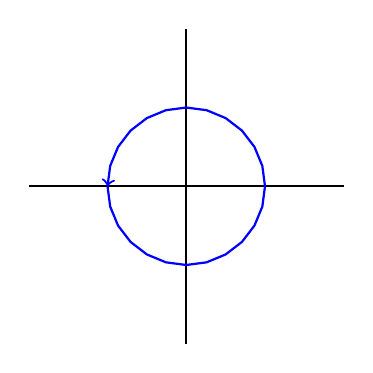
\begin{tikzpicture}
%\draw [help lines,black!20!white] (-1,-1) grid (4,4);

\draw[thick] (0,-2) -- (0,2);
\draw[thick] (-2,0) -- (2,0);

\draw [blue,thick,domain= -180:180, ->] plot ({cos(\x)}, {sin(\x)});

\end{tikzpicture}
\end{center}

\noin the value of $\arg(z)$ increases by $2\pi$, and the value of $\log(z)$ increases by $2\pi i$. The same thing happens with other multivalued functions.

\begin{ex}{}{} What happens to $z^{\frac{1}{2}}$ and $z^{\frac{1}{3}}$ if we travel around the unit circle?

For $z^{\frac{1}{2}}$, we use the formula $\sqrt{r}e^{i\frac{\theta}{2}}$. So, starting at $1$ written as $e^{i0}$, we have $1^{\frac{1}{2}} = 1$. As we move around the circle once (clockwise), we see that $\theta$ moves from $0$ to $2\pi$, and so $z^{\frac{1}{2}}$ moves from $e^{i0} = 1$ to $e^{i\pi} = -1$. Pictorially:

\begin{center}
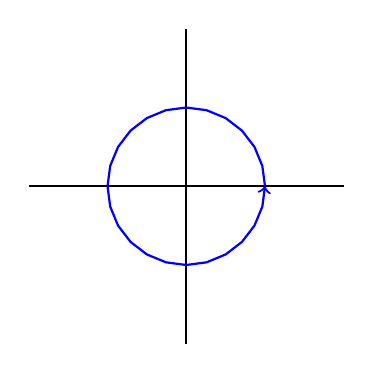
\begin{tikzpicture}[baseline=(current bounding box.center)]
%\draw [help lines,black!20!white] (-1,-1) grid (4,4);

\draw[thick] (0,-2) -- (0,2);
\draw[thick] (-2,0) -- (2,0);

\draw [blue,thick,domain= 0:360, ->] plot ({cos(\x)}, {sin(\x)});

\end{tikzpicture}
\qquad$\longrightarrow$\qquad
\begin{tikzpicture}[baseline=(current bounding box.center)]
%\draw [help lines,black!20!white] (-1,-1) grid (4,4);

\draw[thick] (0,-2) -- (0,2);
\draw[thick] (-2,0) -- (2,0);

\draw [blue,thick,domain= 0:180, ->] plot ({cos(\x)}, {sin(\x)});

\end{tikzpicture}
\end{center}

And to get back to $1$, we need to go around the unit circle twice!

A similar line of reasoning applies to the multi-valued function $z^{\frac{1}{3}}$. In this case, the picture looks like:

\begin{center}
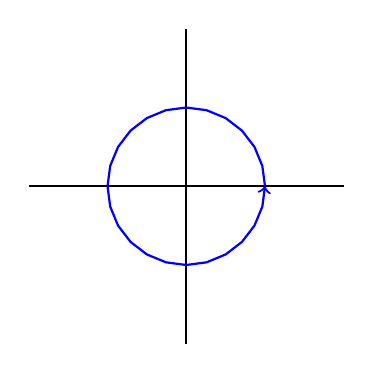
\begin{tikzpicture}[baseline=(current bounding box.center)]
%\draw [help lines,black!20!white] (-1,-1) grid (4,4);

\draw[thick] (0,-2) -- (0,2);
\draw[thick] (-2,0) -- (2,0);

\draw [blue,thick,domain= 0:360, ->] plot ({cos(\x)}, {sin(\x)});

\end{tikzpicture}
\qquad$\longrightarrow$\qquad
\begin{tikzpicture}[baseline=(current bounding box.center)]
%\draw [help lines,black!20!white] (-1,-1) grid (4,4);

\draw[thick] (0,-2) -- (0,2);
\draw[thick] (-2,0) -- (2,0);

\draw [blue,thick,domain= 0:120, ->] plot ({cos(\x)}, {sin(\x)});

\end{tikzpicture}
\end{center}

In this case, as we travel the unit circle once, $z^{\frac{1}{3}}$ goes from $1$ to $\omega_1 = e^{i\frac{2\pi}{3}}$, which is another cube root of unity.
\end{ex}


So what's the solution to this problem? We want to work with continuous functions, if we're going to talk about differentiation. We've seen an example already: for $\log(z)$, we restricted the domain to $\C\setminus (-\infty,0]$, and we were able to find a branch on that domain which is continuous.

This leads us to a more general phenomenon.

\subsection{Branch Cuts}

The idea behind branch cuts is to find a way to take discontinuous branches of a multi-valued function, and to remove a portion of the domain to get a continuous function.

\begin{defbo}{Branch Cuts}{branchcut}\index{Branch!cut} Let $f(z)$ be a branch of a multi-valued function. A branch cut is a curve in $\C$ along which $f(z)$ is discontinuous.\end{defbo}

It is called a branch {\bf cut} because we cut (i.e. remove) the branch cut from the domain to get a continuous function.

\begin{ex}{}{} Let $\log_0(z)$ be the branch of the logarithm given by $\arg(z) \in [-\pi,\pi)$. As we saw earlier, $\log_0(z)$ is discontinuous along $(-\infty,0]$, and so this is a branch cut. Removing $(-\infty,0]$ from the domain of $\log_0(z)$ results in the function $\Log(z)$, which is continuous on its domain.
\end{ex}

All of the multi-valued functions we have seen so far are defined in terms of $\log(z)$ or $\arg(z)$. As such, we can get branch cuts for them by taking branch cuts for $\log(z)$ or $\arg(z)$. Let's start by talking about how to do that.

Consider the branch $\log_0(z)$ of $\log(z)$ given by $\arg(z) \in (\theta, \theta + 2\pi)$ for some $\theta \in \R$. This function is continuous on its domain, in the same way that $\Log(z)$ is continuous on $\C\setminus(-\infty,0]$. We have removed the ray $\{re^{i\theta}|r\ge 0\}$, pictured below:

\begin{center}
\begin{tikzpicture}[baseline=(current bounding box.center)]
%\draw [help lines,black!20!white] (-1,-1) grid (4,4);

\draw[thick] (0,-2) -- (0,2);
\draw[thick] (-2,0) -- (2,0);

\draw[semithick, ->] (0,0) -- (1.3,1.9);

\end{tikzpicture}
\end{center}

\noin By taking this branch cut, we have found a continuous branch. In practice, these are the only types of branch cuts we will consider.

Now that we have a standard way of taking branch cuts for $\log(z)$ or $\arg(z)$, how do these choices affect other multivalued functions?

\begin{ex}{}{} Consider $f(z) = (iz + 1)^{\frac{1}{2}}$, where we are working with the principal branch. What is the branch cut of this function?

Since we are asking about a branch cut, this should serve as a huge clue that this function involves $\log(z)$ somehow. Recall that $(iz+1)^{\frac{1}{2}} = e^{\frac{1}{2}\Log(iz+1)}$.

Now, our branch cut on $\Log(z)$ is to remove $(-\infty,0]$ from the domain. So the corresponding branch cut for $f(z)$ is to remove where $iz + 1 \in (-\infty,0]$.

Suppose $iz + 1 \in (-\infty,0]$. Then $iz \in (-\infty,-1]$. As such, $z\in \left\{\frac{r}{i}|r \le -1\right\} = \{si|s\ge 1\}$. As such, our branch cut is the positive imaginary axis above $1$.
\end{ex}

\section{Infinite Limits and Limits at Infinity}

The last thing to consider is infinite limits and limits at infinity. The key concept here is that in $\C$, there is only one $\infty$. No matter which direction you go out in, left or right, up or down, you get to the same infinity. This is tied to the notion of the Riemann sphere, and of Riemann surfaces, which are a geometric abstraction that makes a lot of complex analysis very nice. We won't be talking in this context in this course. I am pointing these out in case you are interested in further reading.

So, how do we define infinite limits? Well, $f(z)$ should be going to $\infty$. But what way? Well, since all directions give the same $\infty$, any way!

\begin{defbo}{Infinite Limits}{inflim}\index{Limit!infinite}
Let $f:U\rightarrow \C$ and $z_0\in \C$, such that $\{z\in \C| 0 <|z-z_0|< r\} \subset U$ for some $r>0$. Then we say that $\lim_{z\rightarrow z_0} f(z) = \infty$ if:

$$\forall N > 0, \exists \delta > 0 \text{ such that } 0 < |z-z_0| < \delta \implies |f(z)| > N$$
\end{defbo}

In laymans terms, this means that $|f(z)|$ gets arbitrarily large as we get close to $z_0$.

\begin{ex}{}{} Is $\lim_{z\rightarrow 0} e^{\frac{1}{z}}$ infinite or not?

Well, for example, if we consider $z\rightarrow 0$ along the positive real axis, we find that $e^{\frac{1}{x}}$ does go to infinity. After all, $\lim_{x\rightarrow 0^+}\frac{1}{x}=\infty$.

However, consider what occurs as $z\rightarrow 0$ along the positive imaginary axis. We have that $e^{\frac{1}{z}} = e^{\frac{1}{ri}} = e^{\frac{-i}{r}}$. And so $|e^{\frac{1}{z}}| = 1$. As such, if we approach from this direction, $e^{\frac{1}{z}}$ does not approach $\infty$.

So this limit is not infinite.
\end{ex}

What about limits at infinity?

\begin{defbo}{Limits at Infinity}{limatinf}\index{Limit!at infinity}
Let $f:U\rightarrow \C$ such that $\{z\in \C| |z| > r\} \subset U$ for some $r > 0$. Then we say that $\lim_{z\rightarrow \infty} f(z) = L$ if:

$$\forall \varepsilon > 0, \exists M > 0 \text{ such that } |z| > M \implies |f(z) - L| < \varepsilon$$
\end{defbo}

Or, in laymans terms, as $|z|$ gets arbitrarily large, $f(z)$ gets arbitrarily close to $L$.

\begin{ex}{}{} Show that $\lim_{z\rightarrow \infty} z = \infty$.

So, we haven't defined this, but hopefully seeing the two separate definitions allows us to synthesize the correct definition of an infinite limit at infinity.

In this case, we want that as $|z|$ gets arbitrarily large, that $|f(z)| = |z|$ gets arbitrarily large, which is obviously the case.
\end{ex}

\section{The Complex Derivative}

As I have repeatedly mentioned, our goal is to discuss calculus over $\C$. We can finally begin to talk about this! We start with the derivative, which is defined exactly how you would expect:

\begin{defbo}{The Derivative}{derivative}\index{Derivative}
Let $f:U\rightarrow \C$, $z_0\in U$, and $\{z\in\C| |z-z_0|< r\}\subset U$ for some $r > 0$. We say that $f(z)$ is differentiable at $z_0$, with derivative $f'(z_0)$ if:
$$f'(z_0) = \lim_{h\rightarrow 0} \frac{f(z_0 + h) - f(z_0)}{h} \text{\quad exists}$$
\end{defbo}

Before we begin to dive into the theory, let's work out an example.

\begin{ex}{}{} Let $f(z) = iz^2 + 2z$. Find $f'(z)$ from the definition.
\begin{align*}f'(z) &= \lim_{h\rightarrow 0} \frac{i(z+h)^2 + 2(z+h) - (iz^2 + 2z)}{h}\\
&= \lim_{h\rightarrow 0}\frac{i(z^2 + 2zh + h^2) + 2z + 2h - iz^2 - 2z}{h}\\
&= \lim_{h\rightarrow 0} \frac{2izh + h^2 + 2h}{h}\\
&= 2iz + 2
\end{align*}

So $f'(z) = 2iz + 2$, which is what we were expecting.
\end{ex}

Because complex limits are really limits in 2 dimensions, we need to be careful. For example, if you were going to try fo find the derivative of $e^z$ by definition, you would run into some very nasty $\R^2$ limits. We don't want that in our lives. 

However, the solution to avoiding working with nasty $\R^2$ limits is to leverage the 2-dimensional nature of the derivative!

\begin{thmbo}{}{partialder} Suppose $f(z) = u(x,y) + iv(x,y)$ is differentiable at $z_0$. Then the following two equations hold:
$$f'(z) = \frac{\partial u}{\partial x}(x_0,y_0) + i\frac{\partial v}{\partial x}(x_0,y_0)$$
$$f'(z) = \frac{\partial v}{\partial y}(x_0,y_0) - i\frac{\partial u}{\partial y}(x_0,y_0)$$
\end{thmbo}

\begin{proof} Since $f'(z_0)$ exists, we know that $lim_{h\rightarrow 0} \frac{f(z_0 + h) - f(z_0)}{h}$ exists. As such, it must exist from every direction. We will consider approaching along two lines: $h = a + 0i$ and $h = 0 + ib$. I.e., along the real and imaginary axes.

Along the real axis, we get the limit:
\begin{align*}f'(z_0) &= \lim_{a\rightarrow 0} \frac{f(z_0 + a) - f(z_0)}{a}\\
&= \lim_{a\rightarrow 0} \frac{u(x_0+a,y_0) + iv(x_0 + a, y_0) - u(x_0,y_0) - iv(x_0,y_0)}{a}\\
&=\lim_{a\rightarrow 0} \frac{u(x_0+a,y_0) - u(x_0,y_0)}{a} + i\lim_{a\rightarrow 0} \frac{v(x_0 + a, y_0) -v(x_0,y_0)}{a}\\
&= \frac{\partial u}{\partial x}(x_0,y_0) + i\frac{\partial v}{\partial x}(x_0,y_0)
\end{align*}

And along the imaginary axis: 
\begin{align*}f'(z_0) &= \lim_{b\rightarrow 0} \frac{f(z_0 + ib) - f(z_0)}{ib}\\
&= -i\lim_{b\rightarrow 0} \frac{u(x_0,y_0+b) + iv(x_0, y_0+b) - u(x_0,y_0) - iv(x_0,y_0)}{b}\\
&=-i\left(\lim_{b\rightarrow 0} \frac{u(x_0,y_0+b) - u(x_0,y_0)}{b} + i\lim_{b\rightarrow 0} \frac{v(x_0, y_0+b) -v(x_0,y_0)}{b}\right)\\
&= -i\left(\frac{\partial u}{\partial y}(x_0,y_0) + i\frac{\partial v}{\partial y}(x_0,y_0)\right)\\
&=\frac{\partial v}{\partial y}(x_0,y_0) - i\frac{\partial u}{\partial y}(x_0,y_0)
\end{align*}

We therefore have the two expressions for $f'(z_0)$ that we desired.
\end{proof}

Notice, this gives two expressions for the derivative! Since the limit has only one value, we an conclude that these two expressions are actually equal.

\begin{corbo}{The Cauchy-Riemann Equations}{cauchyrie}\index{Cauchy-Riemann}
If $f(z)$ is differentiable at $z_0$, then $f(z)$ satisfies the {\bf Cauchy-Riemann} equations at $z_0$. Namely:
$$u_x = v_y$$
$$u_y = -v_x$$
\end{corbo}

Let's see a couple of examples for how we can use these two results.

\begin{ex}{}{} The principal logarithm $\Log(z)$ is differentiable on $\C\setminus (-\infty,0]$. We will justify why this is true a bit later, but for now we can accept it. Prove that $\Log(z)' = \frac{1}{z}$ where $\RE(z) > 0$.

Let $z = x + iy$. Then $\Log(z) = \ln|z| + i\Arg(z)$. So:
$$u(x,y) = \ln \sqrt{x^2+ y^2}$$
$$v(x,y) = \arctan\left(\frac{y}{x}\right)$$

We know that $f'(z) = u_x + iv_x$. We compute:
\begin{align*}u_x &= \frac{x}{\sqrt{x^2 + y^2}^2}\\
v_x &= \frac{1}{\left(\frac{y}{x}\right)^2 + 1}\left(\frac{-y}{x^2}\right)\\
&= \frac{-y}{\left(\frac{y}{x}\right)^2 + 1}\frac{1}{x^2}\\
&= \frac{-y}{x^2 + y^2}
\end{align*}

As such, the derivative is $\frac{x - iy}{x^2 + y^2} = \frac{\OL{z}}{|z|^2} = \frac{1}{z}$.
\end{ex}

\begin{ex}{}{} Find where $f(z) = \cos(x)$ is differentiable.

We have that $u(x,y) = \cos(x)$ and $v(x,y) = 0$. If this were differentiable, it would satisfy the Cauchy-Riemann equations. We would have:
$$\sin(x) = u_x = v_y = 0$$
$$0 = u_y = -v_x = 0$$

So, this function does not satisfy the Cauchy-Riemann equations when $\sin(x) \ne 0$. I.e, when $x\ne k\pi$.

What happens when $x = k\pi$? Consider:
$$f'(k\pi) = \lim_{a+bi\rightarrow 0} \frac{\cos(k\pi + a) - 1}{a+bi} = \lim_{a+bi\rightarrow 0} \frac{(-1)^k\cos(a) - (-1)^k}{a+bi} $$

Now, since $|a+ib| \ge |a|$, we know that $\left|\frac{(-1)^k\cos(a) - (-1)^k}{a+ib}\right| \le \left|\frac{(-1)^k\cos(a) - (-1)^k}{a}\right|$. Therefore:
$$\lim_{(a,b)\rightarrow (0,0)} \frac{(-1)^k\cos(a) - (-1)^k}{a} = (-1)^k \lim_{a\rightarrow 0} \frac{\cos(a) - 1}{a} = 0$$

\noin by L'Hopital (in $\R$). As such, the squeeze theorem tells us that $\lim_{h\rightarrow 0} \frac{\cos(k\pi + a) - (-1)^k}{a + ib} = 0$.

So $\cos(x)$ is differentiable at exactly the points $z = k\pi$.

\end{ex}

In this example, we saw an example of a function that was differentiable at exactly the places where it satisfied the Cauchy-Riemann equations. Is that generally true? That would make life very nice for us.

\begin{ex}{}{}Consider $f(z) = \sqrt{|xy|}$. Prove that this satisfies the Cauchy-Riemann equations at $0$, but is not differentiable there.

Since $\sqrt{|xy|}$ is real, $u(x,y) = \sqrt{|xy|}$ and $v(x,y) = 0$. Now, computing the partial derivatives using differentiation rules will not work here. We need to use the defintion:
$$u_x(0,0) = \lim_{a\rightarrow 0} \frac{\sqrt{|a\times0|} - \sqrt{|0\times 0|}}{a} = 0$$

And similarly, $u_y = 0$. As such, $u_x = 0 = v_y$ and $u_y = 0 = -v_x$. So $f(z)$ satisfies the Cauchy-Riemann equations at $z = 0$.

However, we need:
$$\lim_{(a,b)\rightarrow (0,0)} \frac{\sqrt{|ab|}}{a + ib}$$

\noin to exist. That means it must exist along every direction! We have shown that it is $0$ along the real and imaginary axes. Consider the direction where $x = y$, and $x > 0$. We get:
$$\lim_{(a,a) \rightarrow (0^+,0^+)} \frac{\sqrt{|a^2|}}{a+ia} = \lim_{a\rightarrow 0^+}\frac{a}{a+ia} = \frac{1}{1+i} \ne 0$$ 

Since we get different limits along different directions, $f'(0)$ does not exist. Therefore, $f$ satisfies the Cauchy-Riemann equations at $z = 0$, but is not differentiable there!
\end{ex}

We would like to have an easy to check, general condition to see if a function is differentiable. The Cauchy-Riemann equations seemed like a good bet, but we've seen that they aren't sufficient to guarantee that a function is differentiable. Can we fix this?

The answer is yes. There is an easy condition we can add, which will salvage the usefulness of the Cauchy-Riemann equations. However, to properly discuss it we will need to take a brief detour into topology.

\subsection{The Topology of $\C$}

Topology is a fairly broad field. Fortunately for us, we will only need some basic definitions. At its most basic, topology is concerned with the notion of an ``open set". For $\C$, these turn out to be fairly nice. They're based on open balls:

\begin{defbo}{Open Ball}{openball}\index{Topology!open ball}
Let $z_0\in \C$. An open ball of radius $r > 0$ centered at $z_0$ is a set:
$$B_r(z_0) = \{z\in \C| |z-z_0|< r\}$$
\end{defbo}

So they're just filled in circles missing their boundaries:

\begin{center}
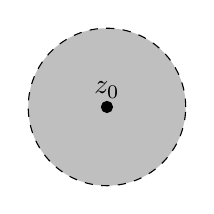
\begin{tikzpicture}

\draw[dashed, fill = lightgray] (1,0) arc (0:360:1);
\draw[fill = black] (0,0) circle (2pt);
\draw (0,0) node[inner sep = -2pt, label = {[label distance = -1pt]90:$z_0$}]{};
\end{tikzpicture}
\end{center}

Open balls are the basic building blocks of open sets. There are two equivalent characterisations:

\begin{defbo}{Open Set}{openset}\index{Topology!open set}
We say that a subset $U \subset \C$ is open if for any $z_0 \in U$, there exists a ball $B_r(z_0)$ which is contained in $U$.

Alternatively, an open set is an arbitrary union of open balls.
\end{defbo}

We can visualize this definition as:

\begin{center}
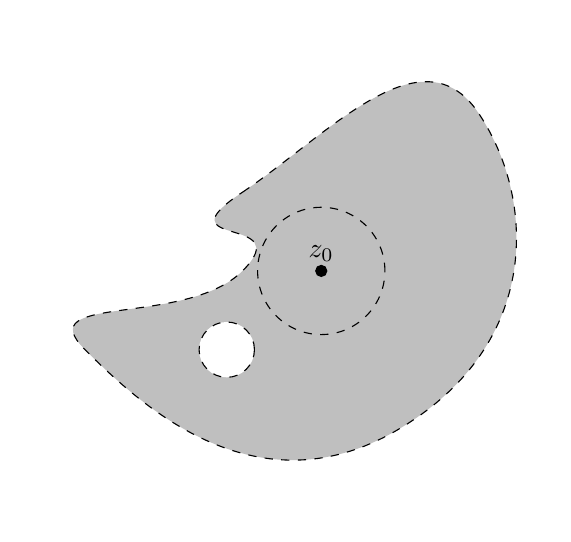
\begin{tikzpicture}
\draw[dashed, fill = lightgray] plot [smooth cycle, tension = 1.3] coordinates {(0,0)  (0,1) (3,2) (2,-2) (-2,-1)};
\draw[dashed, fill = white] (-0.2,-1) circle (10pt);

\draw[fill = black] (1,0) circle (2pt) node[inner sep = -2pt, label = {[label distance = -1pt]90:$z_0$}]{};
\draw[dashed] (1,0) circle (23pt);

\end{tikzpicture}
\end{center}

Notice that around the point $z_0$, we have found a ball $B_r(z_0)$ contained entirely in $U$, which is the shaded region. We could do the same for any point in the shaded region, if we desired.

How do we recognize open sets in practice? If we have a picture, it's easy to do so. The set shouldn't contain any ``edge" or boundary. This is an intuitive notion which is easy to see visually, so we won't go through the effort of describing it formally. There is a formal definition, but it isn't very helpful for developing a visual heuristic.

Algebraically, it's much easier to determine open sets. Open sets are generally described by conditions involving inequalities of some variety. For example: $\{z\in \C| \RE(z) > 1\}$ is an open set. Open balls are open sets. $\C$ and the empty set are open. And there are many other examples.

In addition to open sets, we need one more topological notion: connectedness. The idea behind a set being "connected" is that it is in one piece. To describe this formally, we need to talk about paths.

\begin{defbo}{path}{path}\index{Topology!path}\index{path}A path $\gamma$ in $\C$ is a function $\gamma:[0,1] \rightarrow \C$ such that $\RE(\gamma)$ and $\IM(\gamma)$ are continuous functions.\end{defbo}

In a set that is in one piece, it should be possible to draw a path between two points in the set without leaving the set. And this is precisely the definition of connectedness.

\begin{defbo}{Connected Set}{connectedset}\index{Topology!connected set} A set $U\subset \C$ is called connected if for any two $z_0,z_1\in U$ there exists a path $\gamma$ such that $\gamma(0) = z_0$, $\gamma(1) = z_1$, and $\gamma(t)\in U$ for all $t$.\end{defbo}

Some examples of connected sets:

\begin{center}
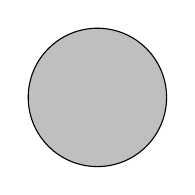
\begin{tikzpicture}[baseline=(current bounding box.center)]

\draw[fill = lightgray] (0,0) circle (25pt);

\end{tikzpicture}
\qquad or \qquad
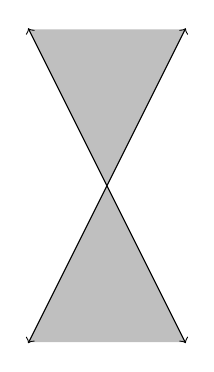
\begin{tikzpicture}[baseline=(current bounding box.center)]

\draw[fill = lightgray, <->] (-1,2) -- (0,0) -- (1,2);
\draw[fill = lightgray, <->] (-1,-2) -- (0,0) -- (1,-2);

\end{tikzpicture}
\qquad or \qquad
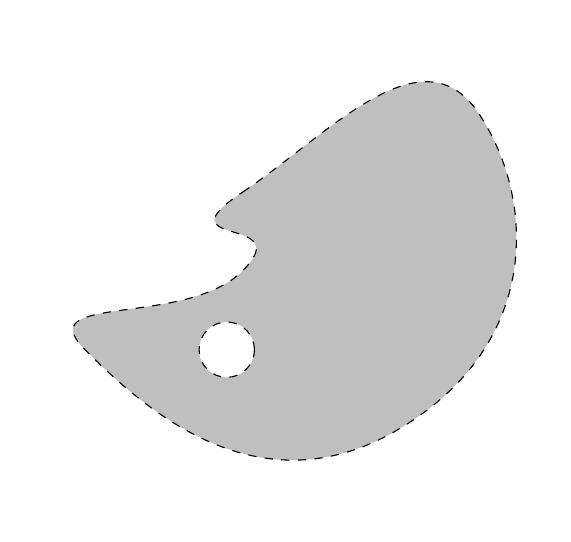
\begin{tikzpicture}[baseline=(current bounding box.center)]


\draw[dashed, fill = lightgray] plot [smooth cycle, tension = 1.3] coordinates {(0,0)  (0,1) (3,2) (2,-2) (-2,-1)};
\draw[dashed, fill = white] (-0.2,-1) circle (10pt);

\end{tikzpicture}

\end{center}

On the other hand, these are sets that are not connected:

\begin{center}
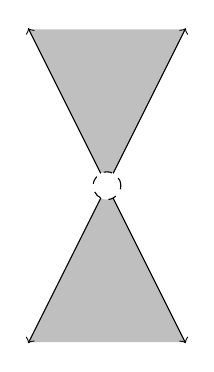
\begin{tikzpicture}[baseline=(current bounding box.center)]

\draw[fill = lightgray, <->] (-1,2) -- (0,0) -- (1,2);
\draw[fill = lightgray, <->] (-1,-2) -- (0,0) -- (1,-2);

\draw[fill = white, dashed] (0,0) circle (5pt);

\end{tikzpicture}
\qquad or \qquad
\begin{tikzpicture}[baseline=(current bounding box.center)]
\draw[fill = CORinner] (-1,0) circle (20pt);
\draw[fill = CORinner] (0,-1) -- (2,2) -- (3.5,0) -- (0,-1);
\end{tikzpicture}
\qquad or \qquad
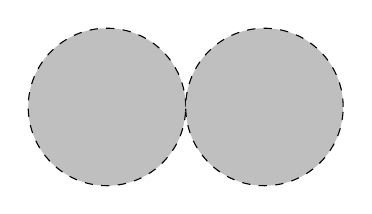
\begin{tikzpicture}[baseline=(current bounding box.center)]
\draw[fill = lightgray, dashed] (-1,0) circle (1);
\draw[fill = lightgray, dashed] (1,0) circle (1);
\end{tikzpicture}
\end{center}

The first of these is hopefully self-explanatory. It's in two pieces. The second of these, which consists of the triangle and the circle, is also in two discrete pieces.

In the third picture, we have open balls which are tangent to one another. However, since they are missing their boundaries, these two sets actually have a gap between them!

Putting these two notions together, we have the basic topological object we will be dealing with in this course:

\begin{defbo}{Domain}{domain}\index{Domain}
A set $U\subset \C$ is called a domain if it is open and connected.
\end{defbo}

\begin{note} This is not the same thing as the domain of a function! You need to be able to tell the difference from context. If we are not discussing a function, then domain will be referring to this definition. In contexts where a function is also being discussed, you will need to be vigilant. There is a difference between the language ``the domain $U$" and ``the domain $U$ of $f$."\end{note}

\begin{note} The last note, while an important technical issue, doesn't quite give the full picture.

In the context of this course, domains will almost only ever occur as the domain of a differentiable function. (In fact, what's called an "analytic function", which we will see soon.)
\end{note}

\subsection{Returning to Differentiation}

Now that we have some topological language, we can get to the point: how do we tell if a function is differentiable?

\begin{defbo}{Holomorphic or Analytic Functions}{holomorph}\index{Analytic Function}\index{Holomorphic Function}
A function $f$ is holomorphic (or analytic) on an open set $U$ if it is differentiable at each point in $U$.

A function $f$ is called holomorphic (or analytic) if it is holomorphic on its domain.
\end{defbo}

\begin{note} Fisher does not use the terminology ``holomorphic" to describe these functions. However, to be precise, analytic really means something different. An analytic function is a function that is equal to a power series.

However, it is one of the crowning achievements of complex analysis that every holomorphic function is analytic. (I.e., if $f$ is differentiable on an open set, then it can be described by power series on that open set.) As such, holomorphic and analytic are the same condition on $\C$. This is not true on $\R$ that differentiable and analytic are the same though, so it is worthwhile to make this distinction.

Plus, I just like the sound of holomorphic more.
\end{note}

So what was the point of introducing all these definitions? Do we get something out of this?

\begin{thmbo}{}{holocond}Suppose $f = u + iv$ is defined on an open set $U$. If $u,v, u_x, u_y, v_x, v_y$ are defined and continuous everywhere in $U$ and $u,v$ satisfy the Cauchy-Riemann equations, then $f$ is holomorphic on $U$.
\end{thmbo}

\begin{proof} The proof of this requires a result from multivariable calculus:

If $u_x$ and $u_y$ are continuous, then $u$ is differentiable. This means that there exists a function $\varepsilon_u(x,y)$ such that:
$$u(x + a,y+b) = u(x,y) + au_x + bu_y  + \varepsilon_u(a,b)$$

\noin The function $\varepsilon_u$ satisfies the condition that:
$$\lim_{(a,b) \rightarrow (0,0)} \frac{\varepsilon_u(a,b)}{\sqrt{a^2 + b^2}} = 0$$

And similarly:
$$v(x + a,y+b) = v(x,y) + av_x + bv_y  + \varepsilon_v(a,b)$$

\noin where $\varepsilon_v$ is defined similarly for $v$.

As such:
\begin{align*}\lim_{a+ib \rightarrow 0} \frac{f(z + h) - f(z)}{h} &= \lim_{a+ib \rightarrow 0} \frac{u(x+a,y+b) + iv(x+a,y+b) - (u(x,y) + iv(x,y))}{a+ib}\\
&= \lim_{a+ib \rightarrow 0} \frac{au_x + bu_y + i(av_x + bv_y) + \varepsilon_u(a,b) + i\varepsilon_v(a,b)}{a+ib}\\
&= \lim_{a+ib \rightarrow 0} \frac{au_x - bv_x + i(av_x + bu_x)}{a + ib} +\lim_{a+ib \rightarrow 0} \frac{\varepsilon_u(a,b) + i\varepsilon_v(a,b)}{a+ib}\\
\end{align*}

Now, $au_x -bv_x + i(av_x + bu_x) = (a+ib)u_x + (ia - b)v_x = (a+ib)u_x + i(a+ib)v_x$. As such:
$$f'(z) = u_x + iv_x  +\lim_{a+ib \rightarrow 0} \frac{\varepsilon_u(a,b) + i\varepsilon_v(a,b)}{a+ib}$$

So we need only consider this last limit. However, note that by the triangle inequality:
$$\left|\frac{\varepsilon_u(a,b) + i\varepsilon_v(a,b)}{a+ib}\right| \le \frac{|\varepsilon_u(a,b)|}{\sqrt{a^2 + b^2}} + \frac{|\varepsilon_v(a,b)|}{\sqrt{a^2 + b^2}}$$

By the definition of $\varepsilon_u$ and $\varepsilon_v$, we know that:
$$\lim_{(a,b)\rightarrow (0,0)} \frac{|\varepsilon_u(a,b)|}{\sqrt{a^2 + b^2}} + \frac{|\varepsilon_v(a,b)|}{\sqrt{a^2 + b^2}} = 0$$

So by the squeeze theorem, $\lim_{a+ib \rightarrow 0} \frac{\varepsilon_u(a,b) + i\varepsilon_v(a,b)}{a+ib} = 0$ as well.

As such, $f'(z) = u_x + iv_x$, and $f$ is differentiable at $z$. Since this applies for any $z\in U$, we see that $f$ is holomorphic on $U$.
\end{proof}


\begin{ex}{}{} Show that $e^z$ is analytic on $\C$.

We need to write $e^z$ as $u + iv$, and show that $u,v, u_x, u_y, v_x, v_y$ are continuous. We also need to show that $u,v$ satisfy the Cauchy-Riemann equations.

To start, $e^z = e^{x}e^{iy} = e^x\cos(y) + ie^x\sin(y)$. As such, $u(x,y) = e^x\cos(y)$ and $v(x,y) = e^x\sin(y)$. These are continuous.

We compute the partials:
$$u_x = e^x\cos(y)$$
$$u_y = -e^x\sin(y)$$
$$v_x = e^x\sin(y)$$
$$v_y = e^x\cos(y)$$


Notice that these are all continuous. And further, that:
$$u_x = e^x\cos(y) = v_y$$
$$u_y = -e^x\sin(y) = -v_x$$

As such, $e^z$ satisfies the conditions of the theorem, and is therefore analytic on $\C$.
\end{ex}

Functions which are analytic on $\C$ are special. They have some very nice properties. For example, their range is always either $\C$ or $\C\setminus\{z_0\}$ for some $z_0\in\C$. This is called Picard's Little Theorem. We won't be using that in this course, but it's a good example of why these functions are special. As such, they have a name:

\begin{defbo}{Entire Function}{entire}\index{Entire Function}
A function which is analytic on $\C$ is called {\bf entire}.
\end{defbo}

We'll talk more about entire functions as the course moves on.

How do we compute derivatives in practice? After all, computing partials and then turning them into a function of $z$ can be quite nasty. Is there a better way?

\begin{thmbo}{The Derivative Rules}{derivrules}
Suppose $f,g$ are differentiable at $z_0$ and $h$ is differentiable at $f(z_0)$. Then:

\begin{itemize}
\item The constant multiple rule: $\omega f(z_0) = \omega f'(z_0)$ for any $\omega \in \C$.
\item The sum rule: $(f+g)'(z_0) = f'(z_0) + g'(z_0)$.
\item The product rule: $(fg)'(z_0) = f'(z_0)g(z_0) + f(z_0)g'(z_0)$.
\item The quotient rule: if $g(z_0) \ne 0$, then $\left(\frac{f}{g}\right)'(z_0) = \frac{f'(z_0)g(z_0) - f(z_0)g'(z_0)}{g(z_0)^2}$.
\item The chain rule: $(h\circ f)'(z_0) = h'(f(z_0))f'(z_0)$.
\end{itemize}
\end{thmbo}

Combining this with the basic derivatives we know: $z$, $e^z$, $\Log(z)$, etc. allows us to figure out the derivatives of basically any function we want.

\begin{ex}{}{} Find the derivative of $z^n$.

Well, we could us the definition of the derivative in combination with the binomial theorem.

Instead, let's use the product rule and induction. We claim that if $f(z) = z^n$, then $f'(z) = nz^{n-1}$ for integers $n \ge 0$.

\paragraph{Base case:} When $n = 0$, we know that $f(z) = 1$, so $f'(z) = 0$. After all, $\frac{f(z + h) - f(z)}{h} = \frac{1-1}{h} = 0$ for $h\ne 0$. So the formula holds when $n = 0$.

For $n = 1$, we have $\lim_{h\rightarrow 0} \frac{(z+h) - z}{h} = \lim_{h\rightarrow 0} \frac{h}{h} = 1$. So the formula also holds for $n = 1$.

\paragraph{Induction hypothesis:} Suppose the derivative of $z^n$ is $nz^{n-1}$ for some $n\ge 0$.

\paragraph{Induction step:} Consider $z^{n+1}$. Let $f(z) = z^n$ and $g(z) = z$. Then, by the product rule:

$$\frac{d\, z^{n+1}}{d\,z} = f'(z)g(z) + f(z)g'(z) = (nz^{n-1})z + z^n(1) = nz^n + z^n = (n+1)z^n = (n+1)z^{(n+1)-1}$$

As such, the formula holds for $n+1$ as well. By induction, our claim holds for all integers $n\ge 0$.

\end{ex}

What about non-integer powers? First, we need to find the derivative of any branch of $\log(z)$.

\begin{ex}{}{} Suppose $\log_0(z)$ is a continuous branch of $\log(z)$, given by taking $\arg(z) \in (\theta,\theta + 2\pi)$. We have already shown that $\Log(z)$ is differentiable. A similar argument will work here. So we'll move ahead with finding the derivative.

We know that $e^{\log_0(z)} = z$. By the chain rule:
$$1 = \frac{d\,z}{d\,z} = \frac{d \, e^{\log_0(z)}}{d\, z} = e^{\log_0(z)}\frac{d\, \log_0(z)}{d\,z}$$

So, $1 = z\frac{d\,\log_0(z)}{d\,z}$. So the derivative of $\log_0(z)$ is $\frac{1}{z}$.
\end{ex}

\begin{ex}{}{} Find the derivative of any branch of $z^{\alpha}$ where $\alpha\in \C$.

By definition, $f(z) = z^{\alpha} = e^{\alpha\log_0(z)}$, where $\log_0(z)$ is the branch of the logarithm corresponding to the branch of $z^{\alpha}$.

By the chain rule, $f'(z) = e^{\alpha \log_0(z)} (\alpha\log_0(z))' = \frac{\alpha e^{\alpha\log_0(z)}}{z}$. Can we simplify this at all?
\begin{align*}\frac{\alpha e^{\alpha\log_0(z)}}{z} &= \frac{\alpha e^{\alpha \log_0(z)}}{e^{\log_0(z)}}\\
&= \alpha e^{\alpha \log_0(z) - \log_0(z)}\\
&= \alpha e^{(\alpha - 1)\log_0(z)}\\
&=\alpha z^{\alpha-1}
\end{align*}

So, the formula we expect works not just for integers, but for any complex exponent.
\end{ex}

\section{Harmonic Functions}

Before we move on, we have one more fact about analytic functions that we're going to discuss. It turns out, they're very closely related to harmonic functions.

\begin{defbo}{Harmonic Function}{harmonic}\index{Harmonic Function}
Let $U$ be an open set in $\C$. A function $u:U\rightarrow \R$ is harmonic if it has continuous second partials $u_{xx}, u_{xy}, u_{yx}$, and $u_{yy}$ and it satisfies that:
$$u_{xx} + u_{yy} =0$$

This is sometimes also written as: $\Delta u = 0$ or $\nabla^2\cdot u = 0$. This is called Laplace's equation.
\end{defbo}

Now, it is a very nice fact about holomorphic functions $f = u + iv$ that $u$ and $v$ are actually second differentiable, and $u_{xy}, u_{yx}, v_{xy},$ and $v_{yx}$ are all continuous. In fact, we will see later that if $f$ is holomorphic, then $f$ is infinitely differentiable. For now, we will take this for granted.

\begin{thmbo}{}{harmonicparts} Suppose $f$ is an analytic function on $U$ and that $u,v$ have continuous second partials. Then $u$ and $v$ are harmonic functions on $U$.\end{thmbo}

\begin{proof} Since $u,v$ have continuous second partials, we know that we can apply Clairaut's theorem to get:
\begin{align*}u_{xx} &= \frac{\partial u_x}{\partial x}\\
& = \frac{\partial v_y}{\partial x} \hspace{40pt} \text{(by C-R)}\\
&= v_{xy} = v_{yx} \hspace{50pt} \text{(by Clairaut)}\\
&= \frac{\partial v_x}{\partial y} = \frac{\partial (-u_y)}{\partial y} \hspace{20pt} \text{(by C-R)}\\
&= -u_{yy}
\end{align*}

So $u_{xx} + u_{yy} = -u_{yy} + u_{yy} = 0$, and $u$ is harmonic. A similar argument shows that $v$ is also harmonic.
\end{proof}

Notice that this proof uses Clairaut's theorem. This is why we need to assume that $u,v$ have continuous second partials. Later on, we will show that all analytic functions have continuous second partials, so this assumption can be dropped.

\begin{ex}{}{} Does there exist a holomorphic function $f = u + iv$ so that $u(x,y) = x^2$?

This theorem tells us that if such a function $f$ exists, then $u(x,y) = x^2$ must be harmonic. However:
$$u_{xx} = 2$$
$$u_{yy} = 0$$

So $\Delta u = 2 \ne 0$. Since $u$ is not harmonic, no such $f$ exists.
\end{ex}

Alright, so the real (and imaginary) parts of an analytic function are harmonic. Is the converse true? I.e., does every harmonic function appear as the real or imaginary part of an analytic function? It turns out that the answer is yes! Let's see an example.

\begin{ex}{}{} Let $u(x,y) = 3x^2y - y^3$. Find an analytic function $f(z)$ whose real part is $u(x,y)$.

First, notice that $u$ is harmonic. We won't use this explicitly anywhere, but our goal is to demonstrate that harmonic functions do appear as the real parts of an analytic function. 

If $f(z)$ is such a function, it must satisfy the Cauchy-Riemann equations. Let $f(z) = u + iv$. Then:
$$v_y = u_x = 6xy$$

As such, we can see that $v(x,y) = \int u_xdy = 3xy^2 + g(x)$ for some function $g(x)$. Why do we get this $g(x)$? Well, we're integrating in terms of $y$. That only recovers $y$ information. In particular, it misses any parts of $v$ that depend only on $x$! So we need to assume there is some part of $v$ that depends only on $x$, and then try to determine what that is.

To do so, let's look at $v_x$. We have $v_x = 3y^2 + g'(x)$. However, by Cauchy-Riemann, we know that:
$$3y^2 + g'(x) = v_x = -u_y = -3x^2 + 3y^2$$

As such, $g'(x) = -3x^2$, and so $g(x) = -x^3 + C$ for some constant $C$.

So, we find that $f(z) = u + iv = (3x^2y - y^3) + i(3xy^2 - x^3 + C) = i(-x^3 -i3x^2y + 3xy^2 +iy^3) + iC$. With some fiddling, one can notice that $x^3 + i3x^2y - 3xy^2 -iy^3 = (x+iy)^3 = z^3$. As such, $f(z) = -iz^3 + iC$ for some $C\in \R$.

\end{ex}

This example turns out to be archetypical. Given $u(x,y)$, finding $v(x,y)$ so that $u+iv$ is analytic boils down to solving a system of partial differential equations. However, the procedure isn't unreasonable. Such $u$ and $v$ are called harmonic conjugates:

\begin{defbo}{Harmonic Conjugates}{harmconj}\index{Harmonic Conjugates}Let $u(x,y)$ be a harmonic function. We say that $v$ is a harmonic conjugate for $u$ if $f(z) = u + iv$ is holomorphic.
\end{defbo}

\begin{ex}{}{} Why do we need this notion? Isn't it true that if $u,v$ are harmonic, then $u+iv$ is holomorphic?

Well, no. Consider $u(x,y) = x$ and $v(x,y) = -y$. Then these are both harmonic. However, $f(z) = x-iy = \OL{z}$, which we know is nowhere differentiable.

So, it is not true that if you take any two arbitrary harmonic functions $u,v$, that $u+iv$ is holomorphic. This is something very special.
\end{ex}

In light of this example, it's natural to ask whether or not harmonic functions even have a harmonic conjugate. The answer is, luckily, yes.	

\begin{thmbo}{}{harmconj} If $u$ is harmonic on an open ball $B$ or on the complex plane $\C$, then there exists a harmonic conjugate $v$ for $u$.
\end{thmbo}

Proving this amounts to solving the system of differential equations:
$$v_y = u_x$$
$$v_x = -u_y$$

Since then $u,v$ satisfy Cauchy-Riemann and $f = u + iv$ will be holomorphic. (We are guaranteed that $u,v$ and their partials are continuous since they are harmonic.) We know $u_x$ and $-u_y$, so we just need to know how to solve the system $v_x = f$ and $v_y = g$. The theoretical idea is to integrate. We will eschew giving a precise proof; our topic isn't PDEs after all.

The condition on the domain of $u$ can be weakened slightly to assume that $u$ is harmonic on a \textit{simply connected domain}. We will define this in the next chapter. Why not just any open set?

\begin{ex}{}{} $\ln(x^2+y^2)$ is harmonic on $\R^2\setminus\{(0,0)\}$ but has no harmonic conjugate on $\R^2\setminus\{(0,0)\}$. Note that $\ln(x^2+y^2)$ is the real part of $2\log(z)$. If it had a harmonic conjugate on $\R^2\setminus\{(0,0)\}$, then $\log(z)$ would have an analytic branch on $\C\setminus\{0\}$, which it does not.
\end{ex}

